\documentclass{article}

\usepackage{amsmath} % math stuff
\usepackage{amssymb} % math stuff
\usepackage{array} % equations and stuff
\usepackage{bm} % bold math
%\usepackage{caption} % suppressed table numbering; incompatible with revtex, and longtable, I think
\usepackage{comment} % comment environment
%\usepackage{enumitem} % customization of enumeration, itemize, and description
\usepackage[T1]{fontenc} % font encoding for special characters, must also use scalable font package
\usepackage[margin=0.8in]{geometry} % paper sizes and margins (but be careful not to mess up pre-defined pages)
\usepackage{graphicx} % for graphics
%\usepackage{helvet} % default font is the helvetica postscript font
\usepackage{layouts} % print units like widths
\usepackage{lipsum} % lorem ipsum filler text
\usepackage{lmodern} % scalable font?
\usepackage{longtable} % multi-page tables
\usepackage{makecell} % specify line-breaks in table cells
\usepackage{mathrsfs} % math script font
%\usepackage{mathtools} % displaystyle for cases environment (dcases)
\usepackage{mhchem} % easier chemical formula
\usepackage{microtype} % allows disabling of ligatures
%\usepackage{newcent} % new century schoolbook font
\usepackage{nicefrac}
\usepackage{parskip} % removes paragraph indentation, and adjusts paragraph skip, as well as list items
\usepackage{pdfpages} % add pdf files as pages
%\usepackage{setspace} % adjust text spacing and indents
\usepackage{siunitx} % decimal alignment
\usepackage{subfigure} % divided figures
%\usepackage{tabu} % extra table options
\usepackage{textcomp} % symbols
\usepackage{threeparttablex} % better footnotes with longtable
\usepackage{titling} % title placement
\usepackage{ulem} % strikethrough text
%\usepackage{url} % superceded by hyperref
\usepackage{verbatim} % verbatim environment
\usepackage{xcolor} % colors and color boxes
\usepackage{xspace} % commands that don't eat up white space
\usepackage{hyperref} % links and page setup; should always come last

\hypersetup{
 bookmarks=true,
 colorlinks=true,
 citecolor=blue,
 linkcolor=blue,
 urlcolor=blue,
 pdfstartview={XYZ null null 1.0} % default open view is 100%
}

\DisableLigatures[f,t]{encoding = T1} % disable ff, fi, fl, tt ligatures, without f option, it also disables -- = endash
\renewcommand{\arraystretch}{1.1} % extra vertical space in tables

\begin{document}

\pagestyle{empty} % don't number pages

% custom title
\begin{center}
{\LARGE Classic Riddler}

\vspace{0.15in}

{\Large 4 December 2020}
\end{center}


\section*{Riddle:}

Three friends are baking holiday cookies together.
They have a flat layer of cookie dough in the shape of an isosceles right triangle (shown below).
They want to design a cookie cutter that will cut out three identical (i.e., congruent) cookies.
The cookies should be as large as possible while staying within the triangle and without overlapping each other.

\begin{center}
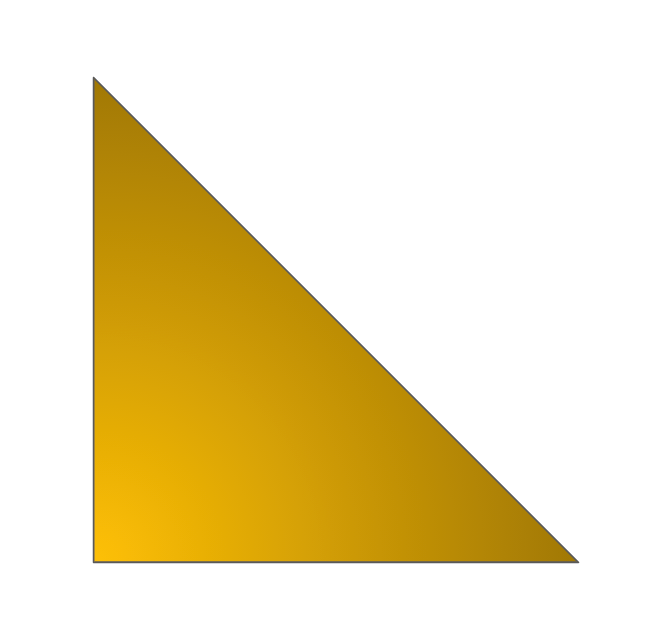
\includegraphics[width=0.5\textwidth]{triangle.png}
\end{center}

Had there been two friends or four friends, they would have been able to use all of the cookie dough.
But with three friends, there will unfortunately be some cookie dough that goes to waste.

What is the greatest percentage of cookie dough that can be made up by the three identical cookies?
When explaining your work, please be as detailed as you can about the arrangement of your cookies so I can verify your work!

\textit{Extra credit}: Instead of a right isosceles triangle, the three friends now want to make identical cookies from a sphinx of cookie dough.
Again, what is the greatest percentage of cookie dough that can go into the three identical cookies?

\section*{Solution:}

Consider the following construction, which is illustrated below.

Let the two corners of the hypotenuse be $B$ and $C$, and the third corner $A$.
Draw the bisector of $\angle BAC$ through the triangle; it intersects $\overline{BC}$ at $D$.
(Equivalently, let $D$ be the midpoint of $\overline{BC}$ and draw the perpendicular bisector of $\overline{BC}$.)
Draw the bisector of $\angle ABD$; it intersects $\overline{AD}$ at $E$.
Draw the bisector of $\angle CAE$; it intersects $\overline{CD}$ at $F$.
Draw the line $\overline{EF}$.

Note that $\triangle ABD$ is congruent to $\triangle ACD$, and $\triangle ABE$ is congruent to $\triangle CAF$.
Therefore $\triangle BDE$ is congruent to $\triangle FDA$; further, $|\overline{DE}|$ is equal to $|\overline{DF}|$.
This means that $\triangle DEF$ is congruent to $\triangle ABC$ (it is isosceles right), so that $\overline{EF}$ is parallel to $\overline{AC}$.
Therefore $\angle DFE$ is equal to $\angle DCA$.
Finally, $\triangle FBE$ is congruent to both $\triangle ABE$ and $\triangle CAF$.

In the diagram below, $\triangle ABE$ is shaded red, $\triangle FBE$ is green, and $\triangle CAF$ is blue.
It shows how much of the original triangle can be cut out, leaving only the un-shaded portion in the middle.

To determine how much of the triangle is cut out (shaded), let the legs of the original triangle be of unit length. 
Then,

\[
|\overline{AB}|=|\overline{AC}|=|\overline{BF}|=1
\]
\[
|\overline{BE}|=|\overline{AF}|=\sqrt{2-\sqrt{2}}
\]
\[
|\overline{AE}|=|\overline{EF}|=|\overline{CF}|=\sqrt{2}-1
\]

With these lengths, the area $\mathcal{A}$ of each cut area is

\[
\mathcal{A}=\frac{\sqrt{6-4\sqrt{2}}}{4}
\]

Summing the three areas and normalizing to the area of the original triangle (\nicefrac{1}{2}), the solution is

\[
\frac{3\mathcal{A}}{\nicefrac{1}{2}}=\frac{3\sqrt{6-4\sqrt{2}}}{2}
\]

or approximately
\fcolorbox{red}{white}{\bf 0.8787}\,.
I don't know if this is the maximum, but it seems pretty good to me.
I'm also noting that this solution depends on the definition of congruent including reflections, which means the cookie cutter must be able to cut from both sides (top and bottom, I guess they would be called).
I'm not even going to attempt the extra credit.

\begin{center}
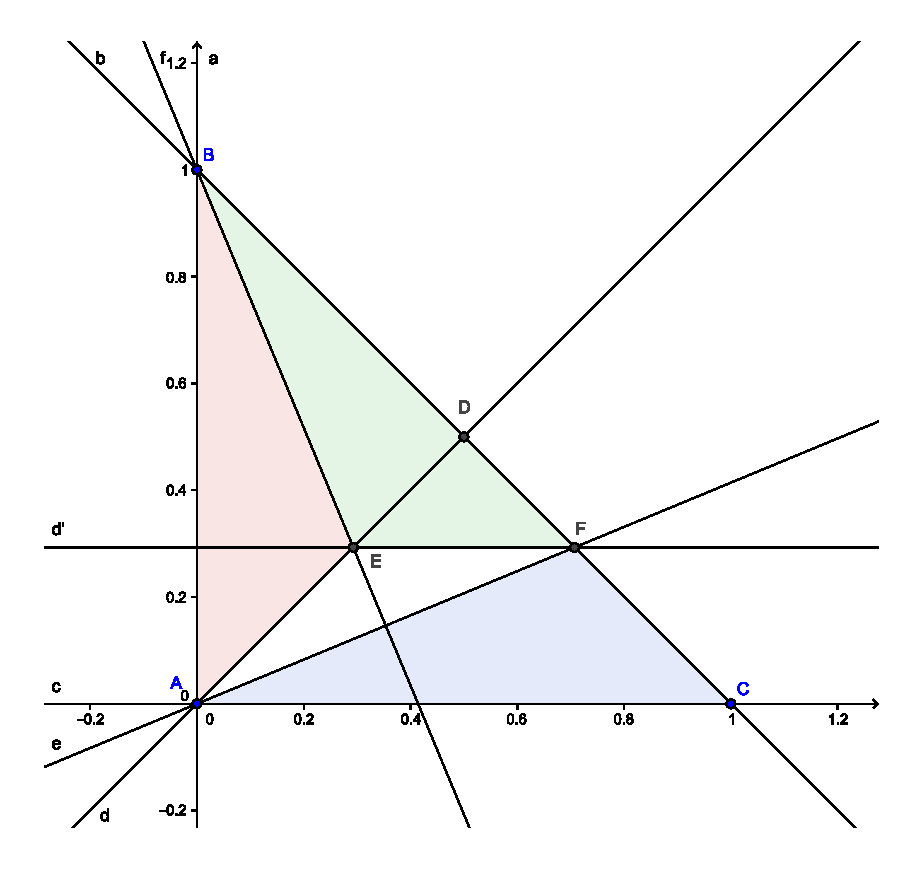
\includegraphics[width=0.7\textwidth]{Construction.pdf}
\end{center}


\end{document}